\Wikidata module is our main proof of concept module which aims to demonstrate the ability of our framework to allow the easy creation of huge modules able to answer to thousand of questions. This module tries to answer to general knowledge using the data stored in \href{http://www.wikidata.org}{\Wikidata}.

\Wikidata is a free knowledge base hosted by the \Wikimedia as a sister project of \Wikipedia. It aims to build a free, collaborative, multilingual structured database of general knowledge (for more information see \cite{42240}). It provides a very good set of API that allows to consume and query \Wikidata content easily. \Wikidata is built upon elements (called items) that are about a given subject. Each item has a label, a description and some aliases to describe it and statements that provides data about this subject.

The \Wikidata module has been written in PHP in order to rely on good libraries that allow to easily interact with the \Wikidata API. Some contributions to these libraries have been done to make them fit better with the module use case. This module works in tree steps:
\begin{enumerate}
    \item It maps \texttt{resource} nodes of the question tree into \Wikidata content: the subjects of \texttt{triple} nodes are mapped to \Wikidata items, predicates to \Wikidata properties and objects to the type of value that is the range of the \Wikidata property of the predicate. If more than one match are possible, a tree per possible match is output.
    \item It performs queries against \Wikidata content using the previously done mapping to reduce as much as possible trees. When we have a \texttt{triple} node where the object is missing the module gets the \Wikidata item of the subject, looks for values for the predicate property and replace the \texttt{triple} node with a \texttt{resource} node for each value of the triple (and so builds as many trees as there are values). When there is a \texttt{triple} node with a missing subject the module uses the \href{http://wdq.wmflabs.org}{WikidataQuery} tool API with \href{https://github.com/ProjetPP/WikidataQueryApi}{a standalone wrapper} built for the project that returns all items with a given statement.
    \item It adds clean text representation of \texttt{resource} nodes added by the previous phase.
\end{enumerate}

The global architecture of the module has been quickly studied by one of the \Wikidata developers that found it fairly good.

\begin{figure}[!ht]
  \centering
    \label{struct}
    \caption{An example output from the \Wikidata module}
    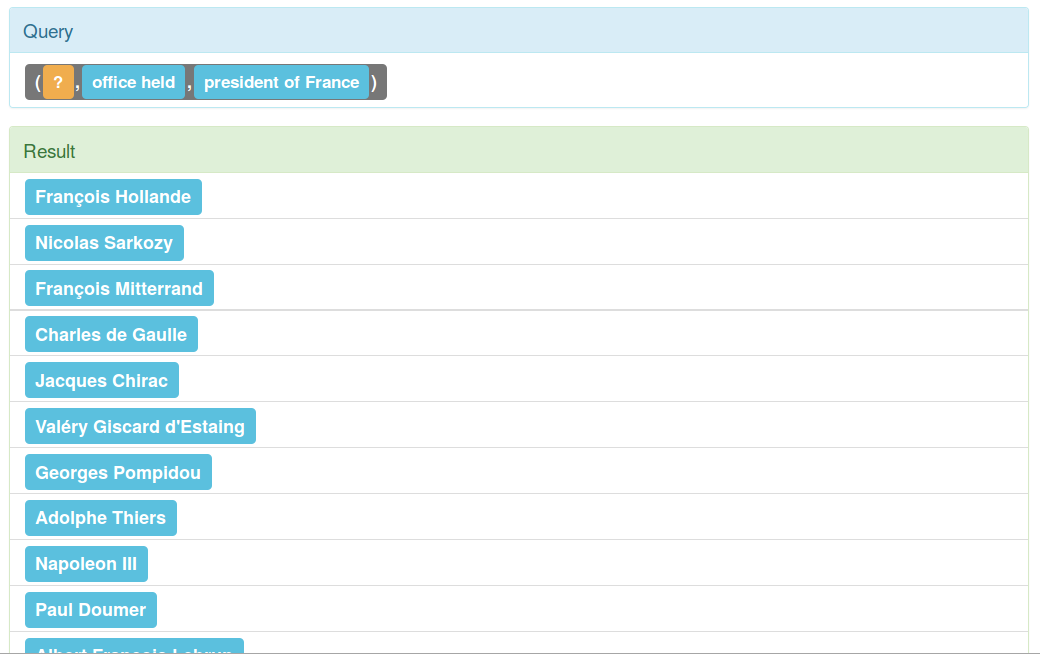
\includegraphics[width=\textwidth]{./wikidata_list_presidents.png}
\end{figure}
